\documentclass{article}\usepackage[utf8]{inputenc}\usepackage[T1]{fontenc}\usepackage{lmodern}\usepackage{amsmath}\usepackage{tikz}\pagestyle{empty}\begin{document}\begin{center}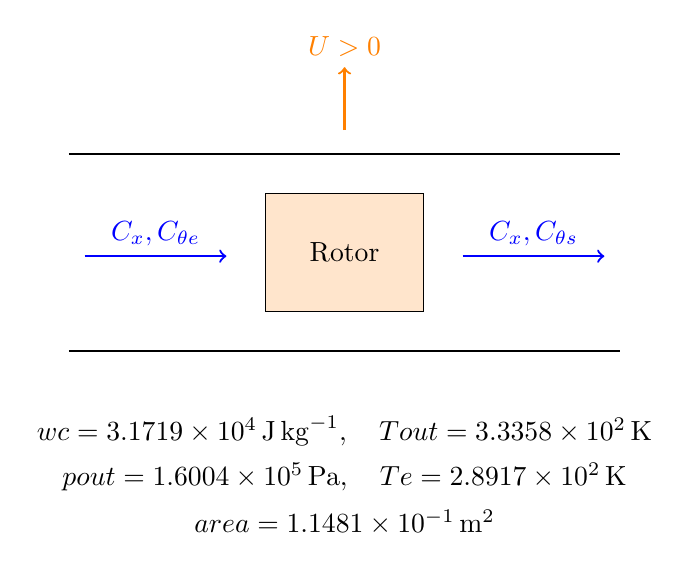
\begin{tikzpicture}\draw[thick] (0,0)--(7,0);\draw[thick] (0,2.5)--(7,2.5);\node[draw,fill=orange!20,minimum width=2cm,minimum height=1.5cm] at (3.5,1.25) {Rotor};\draw[->,blue,thick] (.2,1.2)--(2,1.2) node[midway,above] {$C_x,C_{\theta e}$};\draw[->,blue,thick] (5,1.2)--(6.8,1.2) node[midway,above] {$C_x,C_{\theta s}$};\draw[->,orange,thick] (3.5,2.8)--(3.5,3.6) node[above] {$U>0$};\node[below,align=center] at (3.5,-0.7) {$wc=3.1719\times10^{4}\,\mathrm{J}\,\mathrm{kg}^{-1},\quad Tout=3.3358\times10^{2}\,\mathrm{K}$};\node[below,align=center] at (3.5,-1.2999999999999998) {$pout=1.6004\times10^{5}\,\mathrm{Pa},\quad Te=2.8917\times10^{2}\,\mathrm{K}$};\node[below,align=center] at (3.5,-1.9) {$area=1.1481\times10^{-1}\,\mathrm{m}^{2}$};\end{tikzpicture}\end{center}\end{document}